\section{How data characteristics determine the algorithm}
This section is a methodological explanation and proposed analysis design. Equations define quantities we can compute from the release; they are not new results of the source paper. Implemented examples are in \artifact{scripts/06_motion_examples.py} and \artifact{src/asdmotion_research/temporal.py}.

\subsection{From an image coordinate to a meaningful motion signal}
Let $p_{tj}\in\mathbb R^2$ be joint $j$ at frame $t$, $c_{tj}$ its pose confidence, $f$ the stored frame rate and $\tau$ an analyst-chosen confidence threshold. Define a visibility mask $m_{tj}=\mathbb{1}[c_{tj}\geq\tau]$, additionally requiring finite coordinates. A zero-confidence point is missing measurement, not a physical observation at $(0,0)$.

Let $b_t$ be the shoulder midpoint when both shoulders are visible and let $s$ be the median positive shoulder width over valid frames of the clip. A simple body-relative coordinate is
\[
q_{tj}=\frac{p_{tj}-b_t}{s}.
\]
This removes image translation and a crude body-size/camera-scale factor. It does not correct out-of-plane rotation or perspective, and shoulder width can collapse in profile views. If no valid positive shoulder width exists, the feature is unavailable; do not divide by zero or invent a body scale. Root motion should be kept as a separate channel: subtracting the center can erase informative whole-body rocking or walking. Use joint angles, bone vectors and root displacement as complementary features rather than declaring one normalization universally correct.

For two adjacent valid observations, define normalized velocity $v_{tj}=f(q_{t+1,j}-q_{tj})$. Its units are body scales per second, not metres per second. A mean motion-energy feature over valid adjacent pairs $\mathcal V$ is
\[
E=\frac{1}{|\mathcal V|}\sum_{(t,j)\in\mathcal V}\|v_{tj}\|^2.
\]
If $\mathcal V$ is empty, energy is unavailable. This baseline asks whether a clip simply contains more movement. It cannot decide whether movement is repetitive, purposeful, self-regulatory or clinically significant. Differentiation amplifies pose jitter, so compute velocity only across short valid intervals and compare smoothing choices. Preserve missingness and the fraction of usable time alongside every feature.

\begin{figure}[p]\centering
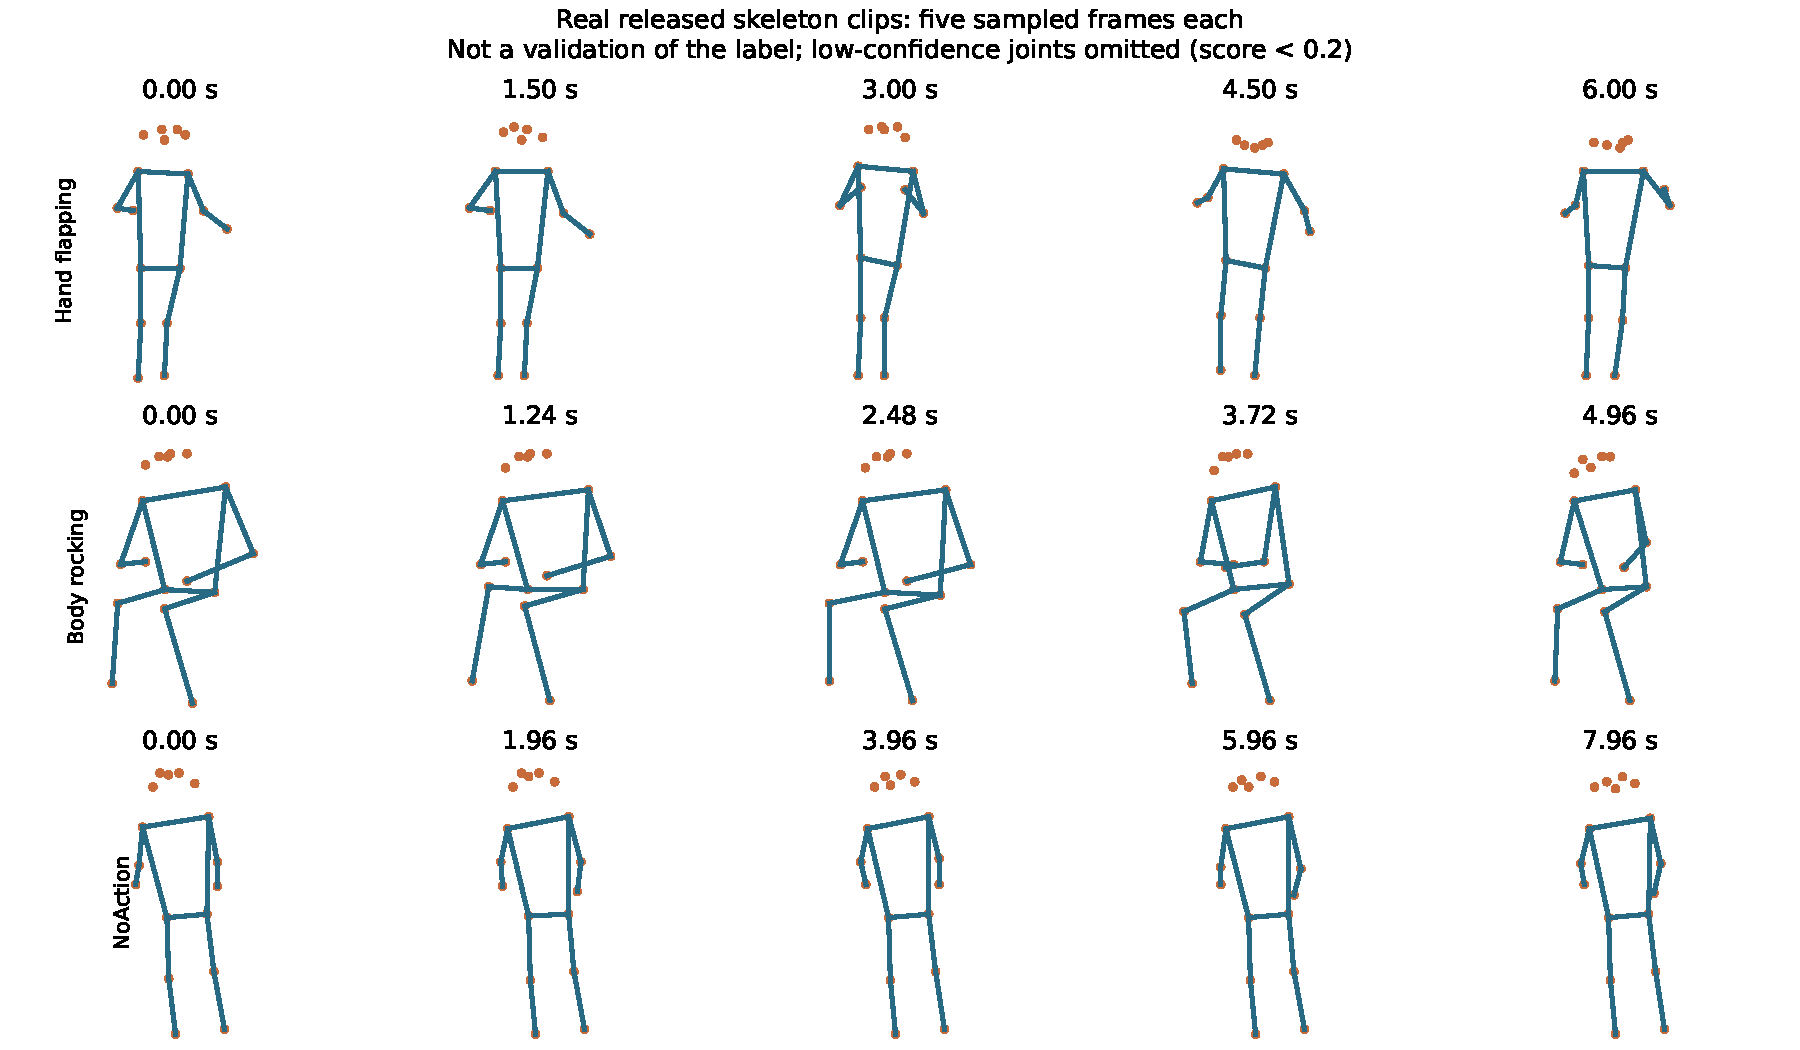
\includegraphics[width=\linewidth]{../../reports/figures/motion_examples.pdf}
\caption{Real skeleton examples selected for relatively good pose confidence, not randomly sampled representatives. Five frames cannot verify repetition or annotation correctness. Exact record identifiers and selection criteria are saved in \texttt{motion\_example\_manifest.json}.}
\end{figure}
\begin{figure}[p]\centering
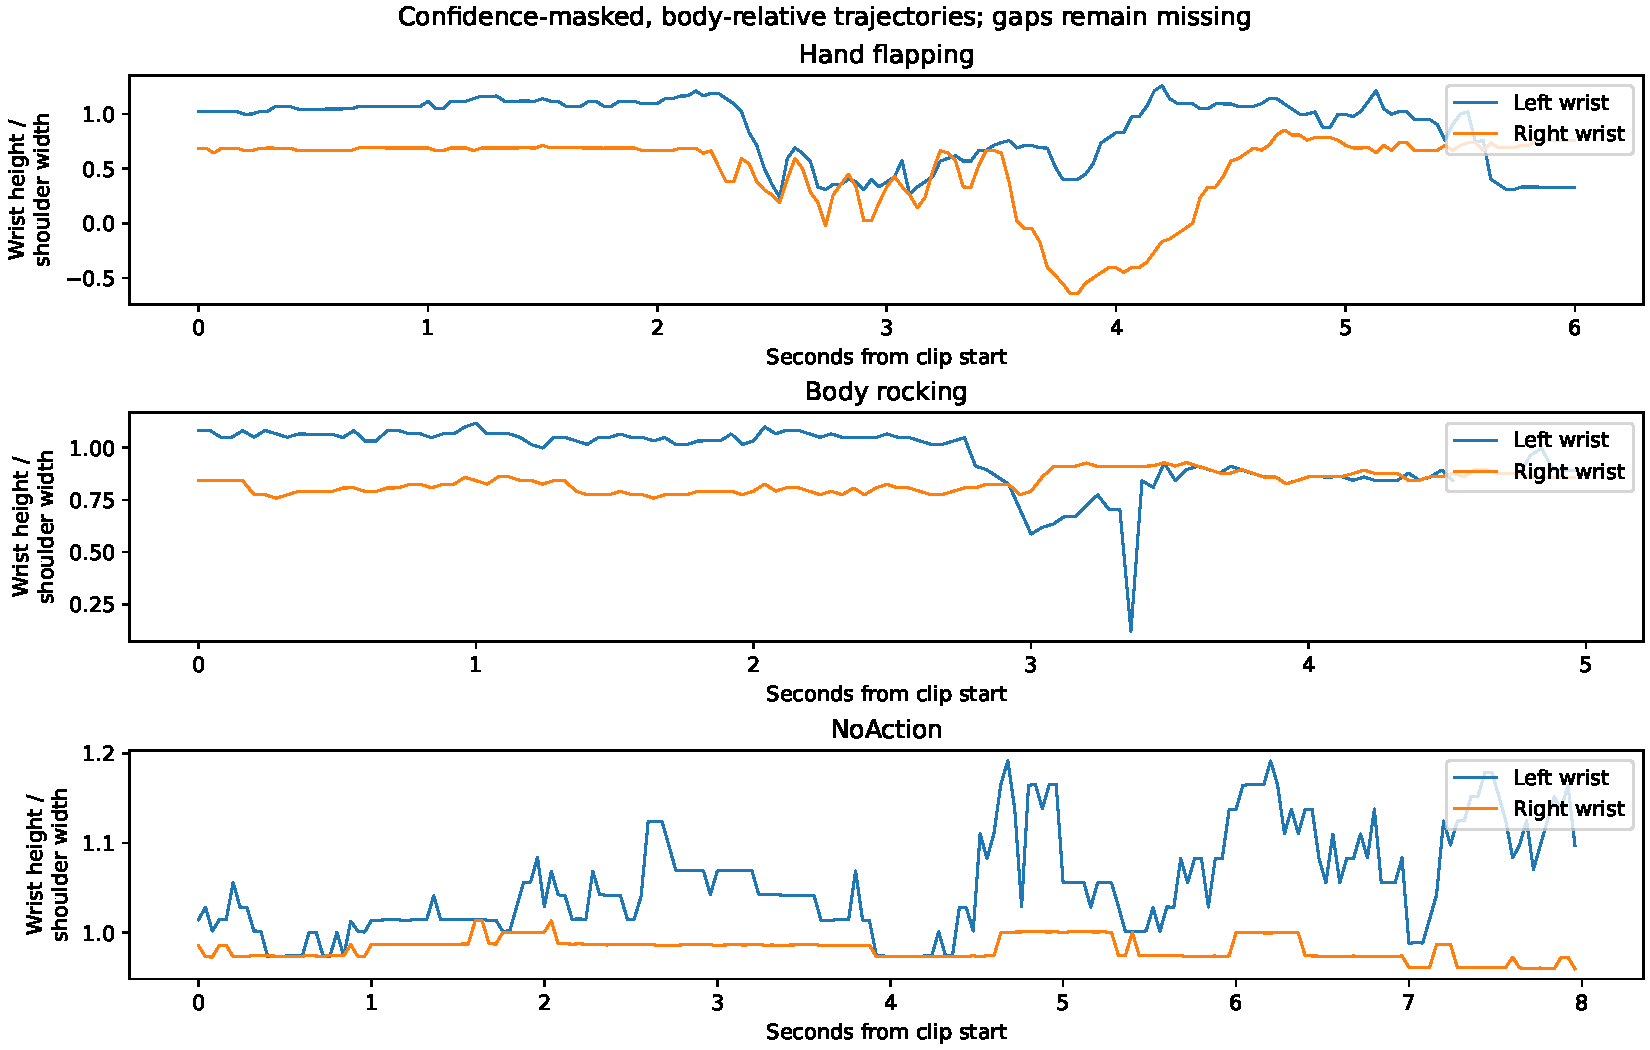
\includegraphics[width=\linewidth]{../../reports/figures/wrist_trajectories.pdf}
\caption{Body-relative wrist traces from the same clips. Missing points remain gaps. Smooth or periodic signals alone do not establish an SMM label; wrist-only features also miss lower-body and subtle finger movements.}
\end{figure}

\subsection{Repetition needs temporal structure, not only magnitude}
Let $x_t$ be one valid, regularly sampled scalar trajectory of $T$ samples, $\bar x$ its mean, and $\ell$ a lag in samples with $0\leq\ell<T$. On a contiguous valid interval with nonzero variance, normalized autocorrelation is
\[
R(\ell)=\frac{\sum_{t=1}^{T-\ell}(x_t-\bar x)(x_{t+\ell}-\bar x)}{\sum_{t=1}^{T}(x_t-\bar x)^2}.
\]
For a constant trajectory the zero denominator makes this normalized quantity undefined, not evidence of rhythmicity. Repeated peaks suggest recurrence; their time spacing is $\ell/f$. A spectrum or autocorrelation can summarize rhythm but is unreliable with few cycles, long missing runs or nonstationary motion. Interpolation through occlusions can manufacture smooth oscillations. Ordinary walking, clapping during a task and repetitive play can also be rhythmic, so periodicity is a candidate feature, not a definition of SMM.

Recurrence analysis instead asks when a trajectory returns to a similar state. Topological methods summarize the geometry of these returns. These may help explain repeated patterns without a large neural network; the recent MBaye study is discussed in the literature section. Whether they distinguish this release's heterogeneous positives from purposeful repetitive negatives is an experiment, not established transfer.

\subsection{Why PoseC3D uses heatmaps}
The source model turns each joint into a spatial confidence blob and stacks these across time. For heatmap pixel $(u,v)$, joint location $(x_{tj},y_{tj})$, confidence $c_{tj}$ and Gaussian width $\sigma$, an illustrative single-person joint heatmap is
\[
H_{tj}(u,v)=c_{tj}\exp\!\left[-\frac{(u-x_{tj})^2+(v-y_{tj})^2}{2\sigma^2}\right].
\]
Spatial convolution can tolerate small coordinate perturbations; temporal convolution learns changes in configuration. The three axes are image width, image height and time. They do not imply depth measurements. The source config uses 17 joint channels and 48 temporally sampled frames, with cropping, resizing and left/right-aware flips.\par
Sources: \artifact{resources/mmaction_template/binary_cfg_template.py}, pinned fork config, Supplement~1, pp.~7--8, and \href{https://openaccess.thecvf.com/content/CVPR2022/html/Duan_Revisiting_Skeleton-Based_Action_Recognition_CVPR_2022_paper.html}{Duan et al., CVPR 2022}, the original PoseC3D method paper archived locally.

This representation fits sparse body motion and avoids modeling appearance directly. It also inherits the pose extractor's failures: a missing wrist has no finger articulation, a wrong child remains wrong, and correlated confidence patterns can become shortcuts. Downsampling a 200-frame window to 48 samples also reduces temporal detail; the same 200 frames correspond to 8 seconds at 25 fps and 6.67 seconds at 30 fps. Equal frame counts are not equal physical durations.

\subsection{Algorithm choices as hypotheses}
\begin{longtable}{@{}P{.20\linewidth}P{.25\linewidth}P{.25\linewidth}P{.22\linewidth}@{}}\toprule
Method & Characteristic used & Why test it & What remains hard\\\midrule\endhead
Energy/angles + logistic model & Motion magnitude, joint geometry & Interpretable, cheap baseline; exposes whether complex models add value & Camera scale, task context and jitter\\
Autocorrelation, spectral or recurrence features & Repetition across time & Tests rhythmic structure beyond movement energy & Irregular bouts, few cycles, purposeful rhythms\\
Temporal convolution/LSTM & Sequential joint features & Learns order and duration with fewer spatial assumptions & Missingness, sampling rate, limited independent subjects\\
ST-GCN / adaptive graph model & Joint/bone relations through time & Explicit body connectivity; useful comparison to heatmaps & Graph depends on accurate joints; appearance/context absent\\
PoseC3D & Confidence-weighted space--time heatmaps & Published reference method and pretrained action representation & Compute, cropping, temporal resolution and quality shortcuts\\
Transformer or self-supervised encoder & Long-range dependencies or reusable motion structure & Later hypothesis when data quality and transfer protocol are stable & Many clips do not equal many independent children; pretraining leakage\\
Quality-aware multi-scale model & Visible-joint masks, multiple durations, uncertainty & Proposed main direction: reliability under heterogeneous missingness & Abstention can selectively exclude the hardest children\\\bottomrule
\end{longtable}
This table proposes a comparison program. It does not assert one model is superior on this release. The original alternative-model results are described separately in the paper section.

\subsection{From a clip score to an event and a session summary}
Let window $i$ cover the half-open frame interval $[a_i,b_i)$ and receive score $s_i$. For frame $t$ with one or more covering windows, the paper's aggregation is
\[
P_t=\max_{i:a_i\leq t<b_i}s_i,\qquad z_t=\mathbb{1}[P_t\geq\theta].
\]
Here $\theta$ is the classification threshold. Frames with no coverage must remain unknown. Taking the maximum means a single positive window raises every frame it covers; this tends to spread a decision over time and can merge neighboring events. Mean pooling, learned temporal localization or hysteresis could behave differently and require validation.\par
Source rule: \cite[p.~4]{barami2024}. Alternative choices are proposed experiments.

\begin{figure}[H]\centering
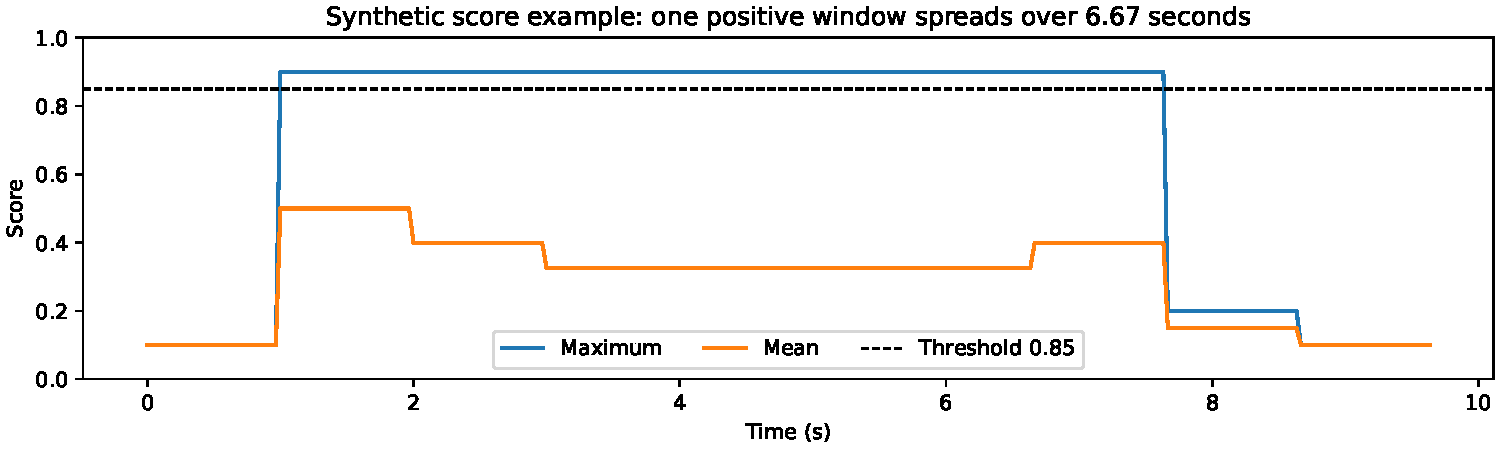
\includegraphics[width=\linewidth]{../../reports/figures/aggregation_demo.pdf}
\caption{Synthetic scores, not measured performance. Maximum and mean aggregation give very different frame decisions from the same windows. The final uncovered frames remain missing.}
\end{figure}

Let $\mathcal O$ contain frames where the child is observable under a predefined quality rule \emph{and} a finite covered prediction exists, and let $\Delta t=1/f$. Define detected time $D=\sum_{t\in\mathcal O}z_t\Delta t$ and observed-and-scored time $O=|\mathcal O|\Delta t$. Observable-and-scored burden is $B=D/O$ when $O>0$. Also report coverage $C=O/T_{\rm recording}$, where $T_{\rm recording}$ is the recording duration in seconds, and distinguish pose-visibility coverage from prediction coverage. A low-coverage recording cannot be treated as confidently low burden. Counting events requires an explicit rule for missing gaps, simultaneous camera views and minimum episode duration. A count per minute is $60N/O$ for event count $N$, with time measured in seconds.

\subsection{Evaluate the intended scientific claim}
\begin{description}[leftmargin=0pt]
\item[Clip discrimination:] precision--recall curves, per-class recall, calibration and quality-stratified errors. Clip accuracy is easily dominated by negatives or acquisition artifacts.
\item[Continuous event detection:] one-to-one episode matching at prespecified temporal intersection-over-union thresholds, onset/offset error, false events per hour and missed events. Frame accuracy alone can conceal clinically relevant errors.
\item[Burden measurement:] absolute and signed duration error, event-count error, agreement plots and observable-time coverage per child. A high correlation can coexist with systematic overestimation.
\item[Generalization:] group by verified child, preserve all sessions/views, tune only on training/validation, and bootstrap children as the independent unit. Site/camera/age/sex analyses require actual metadata and adequate numbers.
\end{description}
These are proposed evaluation requirements. The provided code currently executes release profiling, shortcut diagnostics, source counterexamples and visualization; it does not claim to have run this full predictive benchmark.
